% Training-objective figure v1 (D-129).
% Companion to jan-blockscheme-v4.tex: that figure is the model TOPOLOGY, this one is the
% training PROBLEM on a time axis. Answers input / output / loss / validation.
% Panel (a) draws the horizon ratio to TRUE scale: nf = 400 samples against a 48 000-sample
% record is exactly 1/120, and that ratio is the argument of the figure (figure-style.md S5).
% Style: docs/writeup/figure-style.md (black + black!55 + black!12, no legend, >=Latex, footnotesize).
% Compile: pdflatex training-objective-v1.tex
\documentclass[border=12pt]{standalone}
\usepackage{tikz}
\usetikzlibrary{arrows.meta, calc, decorations.pathreplacing}
\usepackage{amsmath}

% ---- signal shapes (schematic; see caption) --------------------------------
% t in ms. 157 Hz absorber -> 56.52 deg/ms. Slow stage motion -> 7.2 deg/ms.
% The model trace deliberately under-resolves the absorber ripple: that gap is the residual.
\newcommand{\utrace}[1]{1.75 + 0.15*sin(56.52*#1) + 0.11*sin(7.2*#1+40)}
\newcommand{\ydata}[1]{0.15 + 0.16*sin(7.2*#1) + 0.135*sin(56.52*#1)}
\newcommand{\ymodel}[1]{0.15 + 0.16*sin(7.2*#1) + 0.035*sin(56.52*#1+20)}

\begin{document}
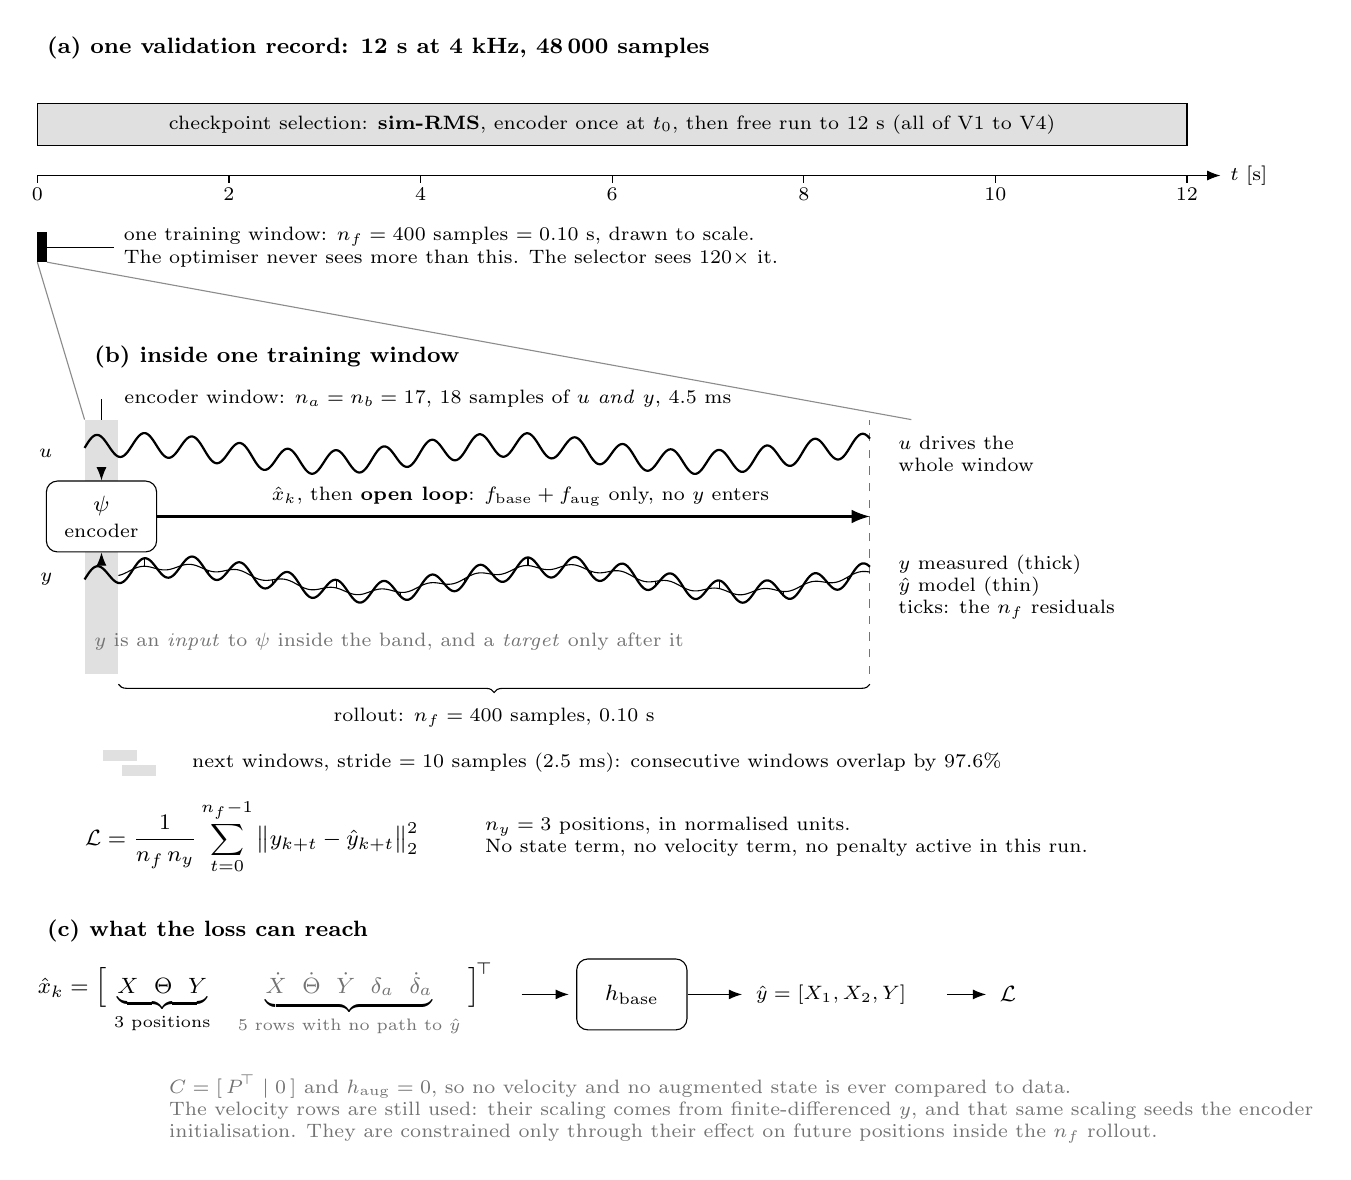
\begin{tikzpicture}[>=Latex, font=\footnotesize,
  small/.style={draw, rounded corners, minimum width=14mm, minimum height=9mm,
                align=center, fill=white},
  ttl/.style={font=\footnotesize\bfseries, anchor=west},
  ann/.style={font=\scriptsize, align=left},
  anc/.style={font=\scriptsize, align=center},
  grey/.style={black!55},
  band/.style={fill=black!12}]

%% ==========================================================================
%% PANEL (a): one validation record, both horizons drawn to TRUE scale
%% ==========================================================================
\begin{scope}[x=1.2167cm]   % 12 s -> 14.6 cm
  \node[ttl] at (0,1.62) {(a) one validation record: 12 s at 4 kHz, 48\,000 samples};

  % selection horizon (above the axis)
  \fill[band] (0,0.38) rectangle (12,0.92);
  \draw       (0,0.38) rectangle (12,0.92);
  \node[anc] at (6,0.65)
    {checkpoint selection: \textbf{sim-RMS}, encoder once at $t_0$, then free run to 12 s
     (all of V1 to V4)};

  % time axis
  \draw[->] (0,0) -- (12.35,0) node[right, font=\scriptsize] {$t$ [s]};
  \foreach \t in {0,2,4,6,8,10,12}{
    \draw (\t,0) -- (\t,-0.10);
    \node[below, font=\scriptsize, inner sep=1.5pt] at (\t,-0.10) {\t};}

  % training horizon (below the axis): 0.10 s of 12 s = 1.2 mm, drawn to scale
  \fill[black] (0,-1.10) rectangle (0.1,-0.72);
  \draw[thin]  (0.1,-0.91) -- (0.80,-0.91);
  \node[ann, anchor=west] at (0.80,-0.91)
    {one training window: $n_f=400$ samples $=0.10$ s, drawn to scale.\\
     The optimiser never sees more than this. The selector sees $120\times$ it.};
\end{scope}

%% magnification wedge into panel (b)
\draw[black!45, thin] (0,-1.10)      -- (0.6,-3.10);
\draw[black!45, thin] (0.1217,-1.10) -- (11.1,-3.10);

%% ==========================================================================
%% PANEL (b): inside one training window     (local x in ms; 110 ms -> 10.5 cm)
%% ==========================================================================
\begin{scope}[xshift=0.6cm, yshift=-5.28cm, x=0.09545cm]
  \node[ttl] at (0,2.98) {(b) inside one training window};

  % encoder window (18 samples = 4.5 ms) and rollout extent, both to scale
  \fill[band] (0,-1.05) rectangle (4.5,2.18);
  \draw[dashed, thin, grey] (104.5,-1.05) -- (104.5,2.18);

  \draw[thin] (2.25,2.18) -- (2.25,2.44);
  \node[ann, anchor=west] at (4.0,2.44)
    {encoder window: $n_a=n_b=17$, 18 samples of $u$ \emph{and} $y$, 4.5 ms};

  % --- u row -------------------------------------------------------------
  \draw[thick] plot[domain=0:104.5, samples=600] (\x, {\utrace{\x}});
  \node[anchor=east, font=\scriptsize] at (-3,1.75) {$u$};
  \node[ann, anchor=west] at (107,1.75) {$u$ drives the\\whole window};

  % --- model chain row ---------------------------------------------------
  \node[small] (psi) at (2.25,0.95) {$\psi$\\{\scriptsize encoder}};
  \draw[->] (2.25,1.50) -- (psi.north);
  \draw[->] (2.25,0.40) -- (psi.south);
  \draw[->, thick] (psi.east) -- (104.5,0.95);
  \node[anc, anchor=south, inner sep=2pt] at (58,1.00)
    {$\hat x_k$, then \textbf{open loop}: $f_{\mathrm{base}}+f_{\mathrm{aug}}$ only, no $y$ enters};

  % --- y row: measured (thick) vs model (thin), residual sticks ----------
  \draw[thick] plot[domain=0:104.5, samples=600] (\x, {\ydata{\x}});
  \draw[thin]  plot[domain=4.5:104.5, samples=580] (\x, {\ymodel{\x}});
  \node[anchor=east, font=\scriptsize] at (-3,0.15) {$y$};
  \foreach \s in {8,16.5,25,33.5,42,50.5,59,67.5,76,84.5,93,101.5}{
    \pgfmathsetmacro{\ya}{\ydata{\s}}
    \pgfmathsetmacro{\yb}{\ymodel{\s}}
    \draw[thin] (\s,\ya) -- (\s,\yb);}
  \node[ann, anchor=west] at (107,0.05)
    {$y$ measured (thick)\\$\hat y$ model (thin)\\ticks: the $n_f$ residuals};
  \node[ann, anchor=west, text=black!55] at (0,-0.64)
    {$y$ is an \emph{input} to $\psi$ inside the band, and a \emph{target} only after it};

  % --- rollout brace -----------------------------------------------------
  \draw[decorate, decoration={brace, amplitude=3pt, mirror}] (4.5,-1.18) -- (104.5,-1.18);
  \node[anc, anchor=north] at (54.5,-1.36) {rollout: $n_f=400$ samples, 0.10 s};

  % --- stride / overlap --------------------------------------------------
  \fill[band] (2.5,-2.16) rectangle (7.0,-2.02);
  \fill[band] (5.0,-2.34) rectangle (9.5,-2.20);
  \node[ann, anchor=west] at (13,-2.18)
    {next windows, stride $=10$ samples (2.5 ms): consecutive windows overlap by 97.6\%};

  % --- the loss ----------------------------------------------------------
  \node[anchor=west, inner sep=0pt] at (0,-3.12)
    {$\displaystyle \mathcal{L}=\frac{1}{n_f\,n_y}\sum_{t=0}^{n_f-1}
      \big\lVert y_{k+t}-\hat y_{k+t}\big\rVert_2^2$};
  \node[ann, anchor=west] at (52,-3.12)
    {$n_y=3$ positions, in normalised units.\\
     No state term, no velocity term, no penalty active in this run.};
\end{scope}

%% ==========================================================================
%% PANEL (c): which state rows the loss can reach
%% ==========================================================================
\begin{scope}[yshift=-10.75cm]
  \node[ttl] at (0,1.15) {(c) what the loss can reach};

  \node[anchor=west, inner sep=0pt] at (0,0.28)
    {$\hat x_k=\Big[\,
      \underbrace{X\ \ \Theta\ \ Y}_{\text{3 positions}}\ \ \
      \underbrace{{\color{black!55}\dot X\ \ \dot\Theta\ \ \dot Y\ \ \delta_a\ \ \dot\delta_a}}
                 _{{\color{black!55}\text{5 rows with no path to }\hat y}}
      \,\Big]^{\!\top}$};

  \draw[->] (6.15,0.35) -- (6.75,0.35);
  \node[small] (hb) at (7.55,0.35) {$h_{\mathrm{base}}$};
  \draw[->] (hb.east) -- (8.95,0.35);
  \node[anchor=west, font=\scriptsize] at (9.00,0.35) {$\hat y=[X_1,X_2,Y]$};
  \draw[->] (11.55,0.35) -- (12.05,0.35);
  \node[anchor=west] at (12.10,0.35) {$\mathcal{L}$};

  \node[ann, anchor=north west, text=black!55] at (1.55,-0.55)
    {$C=[\,P^{\!\top}\;|\;0\,]$ and $h_{\mathrm{aug}}=0$, so no velocity and no augmented state
     is ever compared to data.\\
     The velocity rows are still used: their scaling comes from finite-differenced $y$, and
     that same scaling seeds the encoder\\
     initialisation. They are constrained only through their effect on future positions
     inside the $n_f$ rollout.};
\end{scope}

\end{tikzpicture}
\end{document}

% ---------------------------------------------------------------------------
% SUGGESTED CAPTION (figure-style.md S7: state parameter values and real vs schematic)
%
% The training objective and its two horizons. (a) A validation record is 12 s at 4 kHz
% (48 000 samples). The checkpoint is selected on sim-RMS, a free-run simulation over the
% whole record, while one training window covers nf = 400 samples (0.10 s). Both bars are
% drawn to scale: the trained horizon is 1/120 of the selected horizon. (b) Inside one
% window the encoder consumes 18 samples of u and y (na = nb = 17 plus y(k), 4.5 ms) to set
% the initial state, after which the model runs open loop on u alone; the loss is the mean
% squared output error over the 400 rollout steps, on the three positions in normalised
% units. Windows are cut every stride = 10 samples, so consecutive windows share 97.6% of
% their samples. (c) The output map C = [P^T | 0] with h_aug = 0 means only the three
% position rows reach y_hat: velocities and augmented states are never compared to data and
% are constrained only through their effect on future positions. Traces in (b) are
% schematic. Values are those of the run configured in scripts/gantry/
% gantry_interconnect_dynamic.py (mode = augmentation, fs = 4 kHz, nf_seconds = 0.100,
% stride = 10, nx_ann = 2), for which no parameter, orthogonality or defect penalty is
% active. Model topology is given separately in jan-blockscheme-v4.
% ---------------------------------------------------------------------------
